\chapter{Background Reading}
\label{chap:background-reading}

\section{Synote}
\label{sec:synote}

\subsection{Conventions}
\label{subsec:conventions}

Every developer has their own programming style. When numerous individuals are contributing to a software product over time, it is necessary to provide a contribution document to ensure all developers adhere to the same conventions. Synote's conventions that applied to our development were:

\begin{itemize}
    \item \textbf{Promises over Callbacks} - To make the asynchronous code easier to read and understand.
    \item \textbf{Specific error structure} - A JSON with properties for the thrown error and an appropriate error message.
    \item \textbf{HTML element IDs} - All elements must have an \texttt{id} attribute of the form  \texttt{$<$name$>$\_$<$type$>$} where \texttt{name} is an intuitive name for the element and \texttt{type} corresponds to the type of the element.
    \item \textbf{Server side testing} - Trigger all branches. If a branch cannot be tested it is considered a bug.\\
\end{itemize}

There are several additional conventions found in \texttt{CONTRIBUTING.md} which is a continuously evolving document. New conventions have been introduced as a result of our development, such as the HTML element ID convention and conventions regarding server side testing, which are discussed in \textbf{Chapter \ref{chap:further-work}}.

\section{Payment Systems}
\label{sec:payment-systems}

% Should probably have nomenclature section to define: Merchant, Payment Gateway, Payment Processor, Merchant Account

\subsection{Introduction}
\label{sec:payment-intro}

E-Commerce has existed in various forms since the 1970s with its seminal act being a drug deal between Stanford and MIT students \cite{power-mike-online-highs}. Later that same decade Michael Aldrich demonstrated the first online shopping system. This system was used in 1984 for the first time to buy groceries from Tesco, marking the first true Business-To-Customer online transaction \cite{winterman-kelly-online-shopper}. Since Sir Tim Berners-Lee invented the World Wide Web, E-Commerce has grown substantially with industry revenue in the UK reaching \euro{157 billion} in 2016 \cite{khaksar-2016}.\\

The primary component of E-Commerce is the online payment system. A common approach for such systems is: Merchants collect payment information from customers, then send the information through a payment gateway to a payment processor which in turn pays into a merchant account. The way in which merchants collect payment information is an important concern which is handled in one of the several ways discussed in \textbf{Section \ref{subsec:gathering-payment-data}}.

\subsection{Considerations}
\label{subsec:considerations}

Security is an essential consideration for online payment systems. E-Commerce begins with customers trusting that the system provided by a merchant is \textit{safe} to use. For an online transaction to be considered \textit{safe}, it must be:

\begin{itemize}
	  \item Confidential - Inaccessible to unauthorized parties.
    \item Encrypted - Only decrypted by an authorized party.
    \item Auditable - Recorded to compliant standard.
    \item Non-Repudiable - Undeniable by both sender and recipient.
    \item Authenticated - Access controlled through an authentication mechanism.
    \item of Integrity - Unalterable during transmission.
\end{itemize}

The Payment Card Industry (PCI) Security Standards Council, exists to develop standards which ensure the above criteria are met. The Data Security Standard (DSS) created by the PCI council "provides a baseline of technical and operational requirements designed to protect account data" and "applies to \textit{\textbf{all}} entities involved in payment card processing--including merchants" \cite{PCI-DSS}.\\

PCI DSS is intended to protect cardholder data that is "processed, stored or transmitted by merchants" \cite{PCI-DSS}. The forms of data in question are depicted in \textbf{Figure \ref{fig:card-data}}, each of which have guidelines associated with them regarding storage and protection. Payment gateway services handle most PCI DSS compliance to remove the burden from the merchant but in some cases, not all of it, as described in \textbf{Section \ref{subsec:gathering-payment-data}}.

\begin{figure}[!hbt]
  	\centering
 	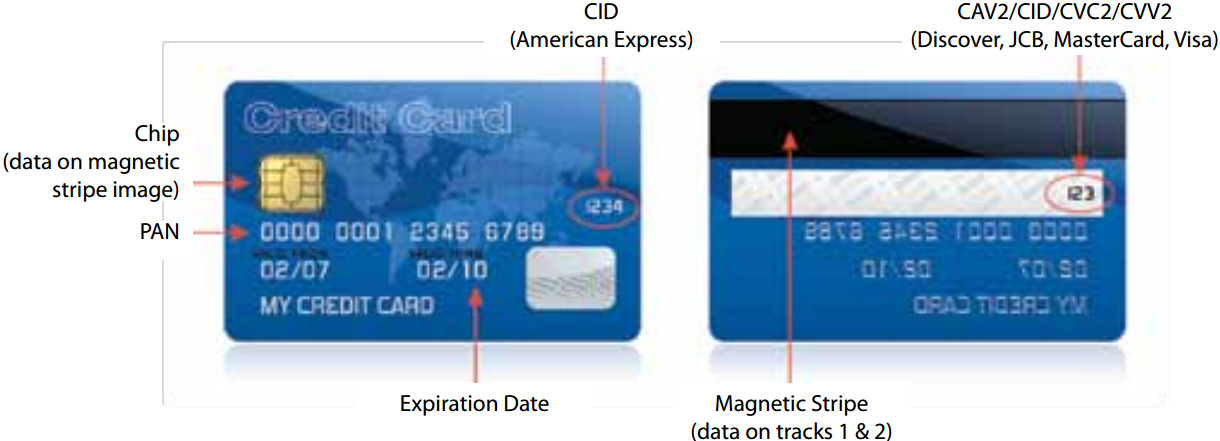
\includegraphics[width=\textwidth]{card-data.png}
  	\caption{Types of Data on a Payment Card\cite{card-data}}
 	\label{fig:card-data}
\end{figure}

\subsubsection{Security}
\label{subsec:security}

Encryption is an essential security measure when transmitting payment information over a network and ensures that only a specified receiver can decrypt the information. PCI DSS dictates the use of Hypertext Transfer Protocol Secure (HTTPS) which use either Secure Sockets Layer (SSL) or Transport Layer Security (TLS) protocols that have an asymmetric Public Key Infrastructure (PKI) system. This means that information can be encrypted with one key at the sender and decrypted by a different key at the receiver or vice-versa \cite{comodo}.\\

To establish a secure connection over HTTPS, an HTTPS/SSL certificate is required, which creates a binding between an organizational identity and a domain name, server name or host name \cite{ssl-certificate}. This certificate is used during a handshake procedure between sender and receiver to establish a secure connection through which payment data may be sent.

\subsection{Gathering Payment Data}
\label{subsec:gathering-payment-data}

The process of collecting a customer's payment information differs between payment gateway providers. The three main methods include:

\begin{enumerate}
	\item Redirection to payment website
    \item Form generated by payment gateway provider
    \item Custom form provided by merchant
\end{enumerate}

Methods 1 \& 2 fully remove the burden of PCI DSS compliance from the merchant as both circumvent processing, storage and transmission on/through the merchants web service. Method 3 however, involves the merchant collecting the payment information, potentially performing validation on the input and sending the information to the payment gateway. It is important to distinguish at this time that the payment information is merely being handled on a client and not sent through the merchants server. To remain compliant with this method, the data has to be encrypted and sent directly through a secure connection to the payment gateway, where it can be tokenized. Such tokens can be processed and stored on a merchant's server in a compliant manner. A collection of payment gateway services and their supported data gathering methods are shown in \textbf{Table \ref{tab:gateway-providers}}. \\

\begin{center}
\begin{tabular}{ |p{3.5cm}|p{1.75cm}|p{2cm}|p{2cm}|  }
 \hline
 	\multicolumn{4}{|c|}{Payment Gateway Services Data Gathering Methods} \\
 \hline
 	\multicolumn{1}{|c|}{Provider} &
 	\multicolumn{1}{|c|}{Redirection} &
 	\multicolumn{1}{|c|}{Generated Form} &
 	\multicolumn{1}{|c|}{Merchant Form}  \\
 \hline
 	Authorize.Net\cite{authorize-net} & \multicolumn{1}{|c|}{Yes} & \multicolumn{1}{|c|}{No} & \multicolumn{1}{|c|}{Yes} \\
 \hline
 	PayPal\cite{paypal} & \multicolumn{1}{|c|}{Yes} & \multicolumn{1}{|c|}{Yes} & \multicolumn{1}{|c|}{Yes (Pro)} \\
 \hline
 	amazon payments\cite{amazon-payments} & \multicolumn{1}{|c|}{Yes} & \multicolumn{1}{|c|}{No} & \multicolumn{1}{|c|}{No} \\
 \hline
    Stripe\cite{stripe} & \multicolumn{1}{|c|}{Yes} & \multicolumn{1}{|c|}{Yes} & \multicolumn{1}{|c|}{Yes} \\
 \hline
 	Braintree (PayPal)\cite{braintree} & \multicolumn{1}{|c|}{Yes} & \multicolumn{1}{|c|}{No} & \multicolumn{1}{|c|}{No} \\
 \hline
\end{tabular}
\captionof{table}{Payment Gateway Providers}
\label{tab:gateway-providers}
\vspace{0.4cm}
\end{center}

\section{Frameworks}
\label{sec:frameworks}

\subsection{Importance of Having Frameworks}
\label{subsec:importance-of-having-frameworks}

In a capsule, a framework can be thought of as an abstraction tool which makes it easier to write applications \cite{1stwebdesigner}. It is essentially a set of integrated software artefacts e.g. common pre-formatted classes and functions which work together to promotes reuse of code \cite{framework-report-vamderbilt}. This in turn improves the productivity of developers since they can focus on implementing desired requirements instead of dealing with the overhead of application infrastructure \cite{cimetrix}. From a business point of view, having re-usability reduces software cost and improves its quality.

\subsection{What Makes a Good Framework?}
\label{subsec:what-makes-a-good-framework}

\begin{itemize}
    \item \textbf{Efficient} - this is the primary purpose of using a framework. Developers should be able to take advantage of pre-built tested functions to implement requirements which would otherwise be complex to achieve from scratch. For example, ASP.NET MVC framework provides libraries and API’s for database access, session and authorisation management which reduces repetitive and tedious tasks \cite{asp.net-team}.
    \item \textbf{Enforces consistent coding style} - forces the developers to adhere to best practices and conventions when coding to produce applications which are flexible and contain less bugs \cite{cimetrix}.
    \item \textbf{Makes discrete components useful} - frameworks should tie together complex components which are difficult to be used on its own and provide a wrapper around them which can be used to achieve desired functionality with ease e.g. LINQ queries in ASP.NET MVC which allows creation of SQL statements with no prior knowledge of SQL syntax \cite{social-msdn}.
    \item \textbf{Follows well recognised coding styles} - using a well know coding style e.g. PHP and Ruby on Rails uses MVC framework, making it efficient and simple to debug because you know exactly where to look for errors and bugs. It also allows separation of application logic from other components e.g. data access layer, views etc. making code management very easy \cite{speckyboy}.
	\item \textbf{Secure and supportive community} - frameworks are typically written by a team of developers and it’s guaranteed to be thoroughly tested before release. Even if you discover a security threat later on, you can contact the community for patches \cite{OSTraining}. The framework’s community should maintain it by releasing regular updates which improve performance, quality and provide new functionality etc. \cite{cimetrix}
	\item \textbf{Easily extendible} - the framework should allow developers to easily implement custom functionality by overriding pre-defined functions. Where this is not possible, it should be compatible in integrating with additional frameworks to achieve desired functionality. \\
\end{itemize}

\subsection{What Makes a Bad Framework?}
\label{subsec:what-makes-a-bad-framework}
\begin{itemize}
 	\item \textbf{Steep learning curve} - An initial learning curve is tolerable if framework brings benefits in the long run. However, it is important to ensure that this learning curve is not too steep that using a framework becomes an overhead instead of an advantage \cite{OSTraining}.
    \item \textbf{Lack of customisation } - it can be difficult to achieve a tailored functionality when framework doesn’t allow over-riding of certain functions. In this case, developer will have to write this functionality independently and integrate it with the framework \cite{Quora}. Difficulty comes in when you have to really understand how the framework works under the hood to “hack” in the functionality.
    \item \textbf{Risk of learning framework, not understanding the language} - Frameworks such as CakePHP allow you to setup a basic site in under 5 minutes. Its scaffolding feature can create controllers, views etc. on the fly with no input from developer. So being able to use a framework doesn't essentially mean that you know the language well \cite{Vizteams}.
    \item \textbf{Risk of being outdated} - If a framework is not regularly maintained e.g. security risks not patched, no performance improvements etc., then its continued use is futile and potentially dangerous to business. Switching to another framework can be extremely expensive if your code base is very large \cite{Quora}.\\
\end{itemize}

\section{Testing}
\label{sec:testing}

\subsection{Unit Testing}
\label{subsec:unit-testing}

Units tests are tests which isolate standalone units or functions of the application to verify their correctness. Easier to be written by developers since understanding of code is required. Correctness is achieved via assertions i.e. statements of conditions and their expected results. To test a function which which identifies season, provided the date and location, a unit test could be; “I expect the answer ‘summer’ for 16th September in Wales. \\

\subsection{Integration Testing}
\label{subsec:unit-testing}

Integration tests are carried out by testers after running Unit tests successfully. They combine independent modules and evaluate them as a group \cite{search-software-quality}. They focus on testing data transfer between independent components. Consider an example test case for checking interface link between Upload and Albums module in:  \textbf{Table \ref{tab:e2eExampleTable}}. \\

\begin{center}
%Column widths dependent on page width/margins
\begin{tabular}{ |p{4cm}|p{4cm}|p{4cm}|  }

 \hline
 	\multicolumn{1}{|c|}{Objective} &
 	\multicolumn{1}{|c|}{Description} &
 	\multicolumn{1}{|c|}{Expected}  \\
 \hline
 	Check interface link between Upload and Albums module & Click the upload button on Upload page, choose an image and click the OK button & User should be redirected to Albums section where uploaded image should be displayed. \\
 \hline

\end{tabular}
\captionof{table}{E2E Test Case}
\label{tab:e2eExampleTable}
\vspace{0.4cm}
\end{center}

\subsection{E2E Testing}
\label{subsec:e2e-testing}

End-to-End tests are carried out after a complete deployment. They focus on testing the application as a whole instead of focusing on specific front end or back end functions by performing tests as to how a real world user might use the application with no understanding of the code base. E2E test cases should focus on testing critical areas such as communication with other systems, database, interfaces etc. \cite{tutorialspoint}. An example E2E test case to verify successful login may include these steps:\\

\begin{enumerate}
	\item Given I go to the “Login” page
    \item Given I enter “Mathew” for username and “Password” for password
    \item Then I should be on the “Home” page
\end{enumerate}

We were asked to carry out E2E tests on the front end and perform Unit and Integration tests on the backend by Synote’s Client.

\section{JavaScript Test Frameworks}
\label{sec:frameworks}

\section{QA Process}
\label{sec:qa-process}
